\documentclass{article}
\usepackage{amssymb}
\usepackage{amsmath}
\usepackage[utf8]{inputenc}
\usepackage{amsfonts}
\usepackage{hyperref}
\usepackage{systeme}
\usepackage{cancel}
\usepackage{graphicx}
\graphicspath{ {./img/} }
\renewcommand{\contentsname}{Indice}

\title{Analisi Matematica}
\author{Alessandro Monticelli}
\date{A.A. 2021/2022}
  
\begin{document}
  
\maketitle
\newpage
\tableofcontents
\newpage
\section*{Introduzione}
    Appunti di Analisi matematica \- corso di Ingegneria e Scienze Informatiche.
\addcontentsline{toc}{section}{Introduzione}
\newpage
    \section{Insiemi}
    \subsection{Definizione}
        Un insieme è una collezione di elementi. Per ogni elemento si può dire se esso appartiene all'insieme, o no.
    \paragraph{Notazioni:}Un \textbf{insieme} si esprime con una \textbf{lettera maiuscola} \{A,B,C,...\}, 
        un \textbf{elemento} si esprime con una \textbf{lettera minuscola}\{a,b,c,...\}.

    \subsection{Concetti di base e operatori}
    \subsubsection{Inclusione}
        \begin{LARGE}
            \begin{equation*}
                A\ \subseteq\ B
            \end{equation*}
        \end{LARGE}
        Tutti gli elementi di A appartengono a B\newline
        
        \subsubsection*{Esempio:}
        
        \begin{LARGE}
            \begin{equation*}
                A\ =\ \{2,5,6,7\}
            \end{equation*}
            \begin{equation*}
                B\ =\ \{1,2,3,4,5,6,7,8,9\}
            \end{equation*}
            \begin{equation*}
                A\ \subseteq\ B
            \end{equation*}
        \end{LARGE}
        Il sottoinsieme si dice \textit{improprio} se A coincide con B, altrimenti si dice \textit{proprio}.

    \subsubsection{Unione}
        \begin{LARGE}
            \begin{equation*}
                A\ \cup\ B
            \end{equation*}
        \end{LARGE}
        Tutti gli elementi del primo insieme e tutti gli elementi del secondo\newline
        
        \subsubsection*{Definizione:}
        
        \begin{LARGE}
            \begin{equation*}
                A\ \cup\ B\ =\ \{x\ |\ x\ \in\ A\ \vee\ x\ \in\ B\}
            \end{equation*}
        \end{LARGE}

        \subsubsection{Intersezione}
        \begin{LARGE}
            \begin{equation*}
                A\ \cap\ B
            \end{equation*}
        \end{LARGE}
        Tutti gli elementi comuni al primo e al secondo insieme\newline
        
        \subsubsection*{Definizione:}
        
        \begin{LARGE}
            \begin{equation*}
                A\ \cap\ B\ =\ \{x\ |\ x\ \in\ A\ \wedge\ x\ \in\ B\}
            \end{equation*}
        \end{LARGE}

        \subsubsection{Differenza}
        \begin{LARGE}
            \begin{equation*}
                A \backslash B
            \end{equation*}
        \end{LARGE}
        Elementi appartenenti \textbf{solo} ad A e non a B\newline
        
        \subsubsection*{Definizione:}
        
        \begin{LARGE}
            \begin{equation*}
                A\ \backslash\ B\ =\ \{x\ |\ x\ \in\ A\ \wedge\ x\ \notin\ B\}
            \end{equation*}
        \end{LARGE}

        \subsubsection*{Osservazione:}

        \begin{Large}
            \begin{equation*}
                A\ \backslash\ B\ \ne\ B\ \backslash\ A
            \end{equation*}
        \end{Large}

        \subsubsection{Differenza Simmetrica}
        \begin{LARGE}
            \begin{equation*}
                A\ \bigtriangleup\ B
            \end{equation*}
        \end{LARGE}
        
        \subsubsection*{Definizione:}
        
        \begin{LARGE}
            \begin{equation*}
                A\ \bigtriangleup\ B\ =\ (A\ \backslash\ B)\ \cup\ (B\ \backslash\ A)
            \end{equation*}
        \end{LARGE}

        \subsubsection*{Osservazione:}

        \begin{Large}
            \begin{equation*}
                A\ \bigtriangleup\ B\ =\ B\ \bigtriangleup\ A
            \end{equation*}
        \end{Large}

        \subsubsection{Prodotto Cartesiano}
        \begin{LARGE}
            \begin{equation*}
                A \times B
            \end{equation*}
        \end{LARGE}
        
        \subsubsection*{Definizione:}
        
        \begin{LARGE}
            \begin{equation*}
                A\ \times\ B = \{(a,b)\ |\ a\ \in\ A\ \wedge\ b\ \in\ B\}
            \end{equation*}
        \end{LARGE}

        \subsubsection*{Osservazione:}

        \begin{Large}
            \begin{equation*}
                (a,b)\ \ne\ (b,a)\ \Rightarrow\ A\ \times\ B\ \ne\ B\ \times\ A
            \end{equation*}
        \end{Large}

        \subsubsection{Insieme Vuoto}
            \textbf{Notazione:}\newline
            \begin{LARGE}
                \begin{equation*}
                    A = \oslash
                \end{equation*}
            \end{LARGE}
 
    \section{Proposizioni}
    \subsection{Definizione}
        Una proposizione è un'affermazione che è falsa o vera e che può implicare altre affermazioni.
        Con $p, q$ proposizioni:

        \begin{LARGE}
            \begin{equation*}
                p \Rightarrow q
            \end{equation*}
        \begin{equation*}
              \Downarrow
        \end{equation*}
        \begin{equation*}
              p\ implica\ q
        \end{equation*}
        \end{LARGE}
        Se $p$ \textit{implica} $q$ e $q$ \textit{implica} $p$ si dicono \textit{equivalenti}\newline
        \begin{LARGE}
            \begin{equation*}
                p\ \iff\ q
            \end{equation*}
        \end{LARGE}
        \subsection{Quantificatori}
            \begin{itemize}
                \item $\forall$ - per ogni
                \item $\exists$ - esiste
                \item $\exists!$ - esiste ed è unico
                \item $\nexists$ - non esiste
            \end{itemize}
        \subsection{Definizioni, teoremi ed enunciati}
        \paragraph{Definizione:\\ }
            Descrizione univoca di un oggetto.
        \paragraph{Teorema:\\ }
            Affermazione che coinvolge oggetti già definiti
        \paragraph{Enunciato:\\ }
            Un affermazione  da dimostrare composta da un'\textit{ipotesi} e da una \textit{tesi}.
        \hfill \break
        \paragraph{Dimostrazione:\\ }
            Una dimostrazione è l'insieme dei passaggi logici e di calcolo che verificano un enunciato.
        
    \subsection{Principio di induzione}
        \subsubsection*{Teorema}
            Sia $p(n)$ un insieme di proposizioni al variare di $n\ \in\ \mathbb{N}$.\\
            Supponiamo che:\\
            \begin{Large}
                \begin{itemize}
                    \item $p(0)$ sia vera
                    \item $\forall\ n\ \in\ \mathbb{N}, p(n)$ vera $\Rightarrow\ p(n\ +\ 1)$ vera. 
                \end{itemize}
            \end{Large}
        \subsubsection*{Esempio}
        Dimostrare:
        \begin{Large}
            \[1+2+3+\cdots+n \Rightarrow \sum_{k=1}^{n}k = \frac{n(n+1)}{2}\] 
        \end{Large}
        \begin{Large}
            \paragraph{Dimostrazione per induzione: \\}
            \begin{equation}
                p(1) \Rightarrow \frac{1(2)}{2} = 1 \Rightarrow vera
            \end{equation}
            \begin{equation}
                    \sum_{k=1}^{n+1}k = \frac{(n+1)(n+2)}{2}\ ?
            \end{equation}
            \begin{equation*}
                \sum_{k=1}^{n+1}k = 1+2+3+\cdots+n+(n+1) = \frac{n(n+1)}{2}+(n+1)=
            \end{equation*}
            \begin{equation*}
                =n+1(\frac{n}{2}+1)=n+1(\frac{n+2}{2})=\frac{(n+1)(n+2)}{2}\ \Rightarrow\ p(n+1)\ vera
            \end{equation*}
            \hfill \break
        \end{Large}
            La proposizione è verificata.
\
    \section{Collezioni}
\subsection{Insiemi Numerici}
    \begin{itemize}
        \item $\mathbb{N} = \text{Numeri Naturali} = \{0,1,2,3,4,\cdots\}$
        \item $\mathbb{Z} = \text{Numeri Interi} = \{-2,-1,0,1,2,\cdots\}$
        \item $\mathbb{Q} = \text{Numeri Razionali} = \{q\ =\ \frac{m}{n},\ m,n \in \mathbb{Z} \land n \neq 0\}$
        \item $\mathbb{R} = \text{Numeri Reali} = \mathbb{Q}\ \cup\ \mathbb{I} = \text{Numeri Razionali } \cup \text{ Numeri Irrazionali}$\footnote{(Decimali illimitati non periodici come $\sqrt{2}, \pi, e$)}\newline 
    \end{itemize}
    \subsubsection*{Teorema}
    \begin{Large}
        \begin{equation*}
            q \in \mathbb{Q} \Rightarrow q^2 \neq 2
        \end{equation*}
    \end{Large}
    \subsubsection*{Dimostrazione}
        Supponiamo \textbf{per assurdo} che $q^2 = 2$.
        Per ipotesi $q = \frac{m}{n},\ m,n \in \mathbb{Z} \land n \neq 0$ e possiamo supporre che
        $\frac{m}{n}$ sia ridotta ai minimi termini.
        \begin{Large}
            \[
                \systeme{q^2=2,q=\frac{m}{n}} 
                    \iff m^2 = 2n^2
                    \Rightarrow m^2\ \text{è pari} \Rightarrow m\ \text{è pari}
                    \Rightarrow m = 2p, p \in \mathbb{Z} \text{ è pari}\Rightarrow\]
            \[
                \Rightarrow n \text{ è pari}\Rightarrow m \text{ ed } n \text{ hanno il fattore } 2 \text{ in comune}.
            \]\newline
        \end{Large}
        \textit{Assurdo} perchè per ipotesi $\frac{m}{n}$ era ridotta ai minimi termini.
\subsection{Assiomi di $\mathbb{R}$}
    $\mathbb{R}$ è un campo, cioè un insieme su cui sono definite due operazioni (+ e $\cdot$) che gode delle seguenti proprietà:

    \begin{itemize}
        \item \textbf{Proprietà associativa}
        \begin{Large}
            \[\forall x,y,z \in \mathbb{R}\]
            \[(x+y)+z = x+(y+z)\]
            \[(x \cdot y)\cdot z = x \cdot (y \cdot z)\]
        \end{Large}
            
        \item \textbf{Proprietà commutiativa}
        \begin{Large}
            \[\forall x,y \in \mathbb{R}\]
            \[x + y = y + x\]
            \[x \cdot y = y \cdot x\]
        \end{Large}
            
        \item \textbf{Proprietà distributiva}
        \begin{Large}
            \[\forall x,y,z \in \mathbb{R},x\cdot(y+z) = x \cdot y + x \cdot z\]
        \end{Large}
        \item $\exists$\textbf{ Elemento neutro}
        \begin{Large}
            \[0+x = x \forall x \in \mathbb{R}\]
            \[1 \cdot x = x \forall x \in \mathbb{R}\]
        \end{Large}
            
        \item $\exists$\textbf{ Opposto}
        \begin{Large}
            \[\forall x \in \mathbb{R},\exists y \in \mathbb{R}\ |\ x + y = 0\]
        \end{Large}
            
        \item $\exists$\textbf{ Reciproco o inverso}
        \begin{Large}
            \[\forall x \in \mathbb{R}, \exists y \in \mathbb{R}\ |\ x \cdot y = 1\]
        \end{Large}
            
        \item \textbf{Assioma d'ordine}\\
            È sempre possibile dire se un numero è maggiore o minore di un altro.
            \[\mathbb{R}\text{ è un campo sempre ordinato}\]
        \item \textbf{Assioma di completezza}\\
            Siano $A$ e $B$ due sottinsiemi separati (cioè $\forall a \in A,\forall b \in b \Rightarrow a \leq b$), 
            allora:
            \begin{Large}
            \[
                \exists x \in \mathbb{R}\ |\ a \leq c \leq b\ \forall\ a \in A, b \in B     
            \]
            \end{Large}
            
            In sostanza, tra due numeri reali esistono infiniti numeri reali.
    \end{itemize}
\subsection{Cardinalità}
\textit{Contare} gli elementi di un insieme significa stabilire una corrispondenza iniettica con un sottoinsieme di $\mathbb{N}$.

\subsubsection*{Esempio}
\begin{Large}
    \[
        \underbrace{A = \{\bullet,\bullet,\bullet\}}_{3 elementi}
    \]
\end{Large}
Se $A$ ha infiniti elementi e può essere messo in corrispondenza biunivoca con $\mathbb{N},\ A$ si dice \textbf{numerabile}
\subsubsection*{Esempio}
    \begin{Large}
    \[A = \{n \in \mathbb{N}\ |\ \text{n è pari} \}\] \newline
    \end{Large}
    \[A \text{ è equipotente a }\mathbb{N}\]
    \[\mathbb{Q} \text{ è numerabile}\]
    \[\mathbb{R} \text{ non è numerabile}\]
\subsection{Proprietà di densità}
    $\mathbb{Q} \text{ e } \mathbb{R} \setminus \mathbb{Q} \text{ sono \textbf{densi} su }\mathbb{R}$.
    \begin{Large}
        \begin{equation*}
            \forall\ a,b \in \mathbb{R},a \le b
        \end{equation*}
        \begin{equation*}
            \exists\ c \in \mathbb{Q}\ |\ a \le c \le b 
        \end{equation*}
    \end{Large}
\subsection{Notazioni}
\begin{Large}
    $\mathbb{R}^{\star} = \mathbb{R} \setminus \{0\}$\newline
    $\mathbb{R}_{+} = \{x \in \mathbb{R}\ |\ x \geq 0\}$\newline
    $\mathbb{R}_{+}^{\star} = \{x \in \mathbb{R}\ |\ x > 0\}$
\end{Large}
\subsection{Massimo e Minimo}
\subsubsection*{Definizioni}
\subsubsection{Massimo}
Sia $A \subseteq \mathbb{R}, A \neq \varnothing$, un numero reale $\lambda$ si dice \textbf{massimo} di $A$ se:
\begin{Large}
    \begin{equation*}
        \lambda \in A, \lambda \geq x \forall x \in A
    \end{equation*}
\end{Large}
\subsubsection{Minimo}
Sia $A \subseteq \mathbb{R}, A \neq \varnothing$, un numero reale $\mu$ si dice \textbf{minimo} di $A$ se:
\begin{Large}
    \begin{equation*}
        \mu \in A, \mu \leq x \forall x \in A
    \end{equation*}
\end{Large}
\subsubsection*{Esempi}

    \begin{itemize}
    \item
    \[
        A = \mathbb{R}_{+}    
    \]
    \[
        \exists\ \min{A} = 0,\ \nexists\ \max{A}    
    \]

    \item
    \[
        A = \{\frac{1}{n}\ |\ n\in \mathbb{N}\setminus\{0\}\}
    \]
    \[
        \exists\ \max{A} = 1,\ \nexists\ \min{A}    
    \]
    \newline
    infatti: \[
        \frac{1}{n+1} < \frac{1}{n}
    \]
    \newline
    \item
    \[
        A = \mathbb{R}_{+}^{\star}    
    \]
    \[
        \nexists\ \min{A}, \nexists\ \max{A}    
    \]
    \newline
    Infatti se $x \in A$:
    \[
        \frac{x}{2} \in A,\ \frac{x}{2} < x\ \forall x \in A    
    \]
    \end{itemize}
    \subsection{Maggioranti e Minoranti}
    \subsubsection{Maggiorante}
    \subsubsection*{Definizione}
    Sia $A \subseteq \mathbb{R}, A \neq \varnothing$, diciamo che $\lambda \in \mathbb{R}$ è un \textbf{maggiorante} di $A$ se:
    \begin{Large}
        \[
            \lambda \geq x\ \forall\ x \in A    
        \]
    \end{Large}
    \subsubsection{Minorante}
    \subsubsection*{Definizione}
    Sia $A \subseteq \mathbb{R}, A \neq \varnothing$, diciamo che $\mu \in \mathbb{R}$ è un \textbf{minorante} di $A$ se:
    \begin{Large}
        \[
            \mu \leq x\ \forall\ x \in A
        \]
    \end{Large}
    \subsubsection*{Definizione}
    Se $A$ ammette un maggiorante allora si dice \textbf{superiormente limitato}, se ammette un minorante
    si dice \textbf{inferiormente limitato}. Se ammette entrambi si dice \textbf{limitato}.

    \subsubsection*{Osservazione}
    Finito $\Rightarrow$ limitato, limitato $\neq$ finito
    \subsubsection*{Teorema}
    Sia $A \subseteq \mathbb{R}, A \neq \varnothing$
    \begin{itemize}
        \item Sia $A$ sup.\ limitato $\Rightarrow$ l'insieme dei maggioranti ammette minimo
        \item Sia $A$ inf.\ limitato $\Rightarrow$ l'insieme dei minoranti ammette massimo.
    \end{itemize}
    \subsubsection*{Osservazione}
    Se un insieme ammette massimo o minimo, esso è unico.
    \subsubsection*{Definizione}
    Se $A$ è sup.\ limitato chiamo \textbf{estremo superiore} di $A$ (sup.$A$) il minimo dell'insieme
    dei maggioranti, e viceversa (inf.$A$).
    Se $A$ non è sup.\ limitato, poniamo sup.$A = + \infty$ e analogamente $-\infty$ se non è inf.\ limitato.
    \subsubsection*{Esempio}
    \begin{Large}
        \[
            A = \{x \in \mathbb{R}\ |\ 0 \leq x \leq 3\}
        \]
        \[
            \inf{A} = \min{A} = 0
            \sup{A} = 3,\ \nexists\ \max{A}     
        \]
    \end{Large}
\subsection{Intervalli di $\mathbb{R}$}
\begin{Large}
\begin{itemize}
    \item $(a,b) = ]a,b[= \{x \in \mathbb{R}\ |\ a < x < b\}$
    \item $[a,b]=\{x \in \mathbb{R}\ |\ a \leq x \leq b\}$
    \item $(a,b] = \{x \in \mathbb{R}\ |\ a < x \leq b\})$
    \item $(a,+\infty) = \{x \in \mathbb{R}\ |\ x > a\}$
    \item $(-\infty,b) = \{x \in \mathbb{R}\ |\ x < b \}$
\end{itemize}
\end{Large}
Questi insiemi sono \textit{intervalli} in quanto soddisfano la seguente proprietà:
\subsubsection*{Definizione}
Sia $A\subseteq\mathbb{R}$, diciamo che $A$ è un intervallo se\\
\begin{Large}
    \[
    \forall\ c,d \in A, \forall\ h \in \mathbb{R}\ |\ c \leq h \leq d \Rightarrow h \in A
    \]
\end{Large}
\subsubsection*{Esempi}
\begin{itemize}
    \item $(2,3)$ è un intervallo
    \item $(2,3) \cup (4,5)$ non è un intervallo in quanto esso non comprende i valori compresi tra $3$ e $4$.
\end{itemize}
\subsubsection{Punto interno di un intervallo}
\subsubsection*{Definizione}
Sia $I$ intervallo di $\mathbb{R}$, diciamo che $c$ è un punto interno di $I$ quando $c \in I$ ma $c$ non è estremo,
cioè $c \in I \setminus \{\inf{I}, \sup{I}\}$\\
$I = (a,b)=[a,b]\setminus\{a,b\}$
L'insieme dei punti interni si definisce $\mathring{I}$
\subsubsection{Tipi di intervalli}
\begin{itemize}
    \item \textbf{Limitato} se sono presenti maggiorante e minorante
    \item \textbf{Aperto} se $I = \mathring{I}$
    \item \textbf{chiuso} $[a,b]$ 
\end{itemize}
\subsection{Simmetria}
\subsubsection*{Definizione}
$A \subseteq \mathbb{R}$ è simmetrico rispetto all'origine se $x \in A \Rightarrow -x \in A$
\subsubsection*{Esempio}
$(-a,a)$
\subsection{Periodicità}
\subsubsection*{Definizione}
Sia $T \subseteq \mathbb{R}_{+}^{\star}$, sia $A \subseteq \mathbb{R}$ diciamo che $A$ è $T-periodico$ se\\
\begin{Large}
    \begin{equation*}
        \forall\ x \in A, \forall\ x \in \mathbb{Z} \Rightarrow x + kT \in A
    \end{equation*}
\end{Large}

    \section{Funzioni}
\subsection{Definizione}
Siano $A$ e $B$ due insiemi, $A,B \neq \varnothing$, chiamiamo \textbf{funzione} $f$ da $A$ a $B$
una legge che ad ogni elemento di $A$ associa uno ed un solo elemento di $B$
\begin{Large}
    \[
        \forall x \in A, \exists! y \in B\ |\ y = f(x)    
    \]
    \vspace{-1em}
    \[
        f: \underbrace{A}_{\{Dominio\}} \rightarrow \underbrace{B}_{\{Codominio\}}
    \]
\end{Large}
\subsubsection*{Esempio}
    \begin{Large}
        \[
            f: \mathbb{R} \rightarrow \mathbb{R}    
        \]
        \[
            f(x) = 2x    
        \]
    \end{Large}
    oppure
    \begin{Large}
        \[
            f: \mathbb{R} \rightarrow \mathbb{R}
        \]
        \[
            x \mapsto 2x
        \]
    \end{Large}

\subsection{Grafico}
    Il grafico di una funzione è un sottoinsime del \textbf{prodotto cartesiano} tra $A$ e $B$.
    \begin{Large}
        \[
            f:A \rightarrow B
        \]
        \[
            Graf_{f}= \{(x,y) \in A \times B\ |\ y=f(x)\}
        \]
    \end{Large}
\subsection{Iniettività e Suriettività}
    \subsubsection*{Definizione}
        Diciamo che $f:A\rightarrow B$ è \textbf{suriettiva} se l'immagine (sottoinsime del codominio) coincide
        con il codominio
        \begin{large}
            \[
                \forall\ y \in B, \exists\ x \in A\ |\ y = f(x)    
            \]
            \[
                f:A \rightarrow B
            \]
        \end{large}
        \vspace{-7ex}
        \begin{center}
            \begin{small}
                \hspace{0.5cm}$su$
            \end{small}
        \end{center}
    \subsubsection*{Definizione}
        Diciamo che $f:A\rightarrow B$ è \textbf{iniettiva} se:
        \begin{large}
            \[
                \forall\ y \in f(A), \exists! x\ \in A\ |\ y = f(x)    
            \]
            \[
                f:A \rightarrow B    
            \]
        \end{large}
        \vspace{-7ex}
        \begin{center}
            \begin{small}
                \hspace{0.5cm}$|\text{\hspace{-0.1cm}}-\text{\hspace{-0.1cm}}|$
            \end{small}
        \end{center}
    \subsubsection*{Definizione}
        Diciamo che $f:A\rightarrow B$ è \textbf{biunivoca} (o biiettiva o invertibile) se è sia suriettiva che iniettiva.

    \subsubsection*{Esempio}
        \[f: \mathbb{R} \rightarrow \mathbb{R}\]
        \[f(x) = x^{2}\]

        $f$ non è suriettiva perchè non assume valori negativi, quindi non copre tutto il codominio $\mathbb{R}$.
        $f$ non è iniettiva perchè per ogni $x > 0$ esiste più di una $y$

    \subsubsection*{Definizione}
        Sia $f: A\rightarrow B$ biunivoca, chiamiamo funzione \textbf{inversa} di $f$ (indicandola con $f^{-1}$ la funzione:
        \begin{Large}
            \[
                f:B \rightarrow A)
            \]
            \[
                \forall\ y \in B,\ f^{-1}(y) = y = f(x)    
            \]
        \end{Large}
\subsection{Composizione di funzioni}
    \subsubsection*{Definizione}
        Siano $X,Y,Z,W$ insiemi $\neq \oslash$,
        \[f:X \rightarrow Y, g:Z\rightarrow W\ |\ f(X) \subseteq Z\]
        chiamiamo \textbf{funzione composta} $g \circ f$ la funzione:
        \begin{Large}
        \[
            g \circ f: X \rightarrow W, (g \circ f)(x) = g(f(x)),\ \forall\ x \in X 
        \]
        \end{Large}
\subsubsection*{Esempio}
    \begin{Large}
        \[
            f : \mathbb{R} \rightarrow \mathbb{R}, f(x) = 2x + 1
        \]
        \[
            g : \mathbb{R} \rightarrow \mathbb{R}, g(y) = y^{2}
        \]
        \[
            (g \circ f)(x) = g(f(x)) = g(2x + 1) = {(2x + 1)}^{2} = 4x^{2} + 4x +1    
        \]
        \[
            (f \circ g)(y) = f(g(y)) = f(y^{2}) = 2y^{2} + 1
        \]
        \[
            g \circ f \neq f \circ g    
        \]
    \end{Large}
\subsection{Funzione identità}
    \begin{Large}
        \[
            f \circ f^{-1} = f^{-1} \circ f = Id    
        \]
        \[
            Id(x) = x    
        \]
    \end{Large}
    \subsubsection*{Teorema}
        Siano $f: X \rightarrow Y, g: Z \rightarrow W$ invertibili, $Y = Z \Rightarrow g \circ f$ è invertibile 
        e ${(g \circ f)}^{-1} = f^{-1} \circ g^{-1}$.

\subsection{Funzioni di una variabile reale}
    Sia $c \subseteq \mathbb{R}, f:A \rightarrow \mathbb{R}$
    \subsubsection*{Esempi}
        \begin{itemize}
            \item $f(x) = 2x + 1$
            \item $f(x) = |x|$
            \item $f(x) = sgn(x)$
            \item $f(x) = [x]$
        \end{itemize}
    \subsubsection*{Definizione}
        Sia $f:A\rightarrow \mathbb{R}, A \subseteq \mathbb{R}$, diciamo che $f$ è limitata se lo è $f(A)$.
        \begin{Large}
            \[
                \sup{f} = \sup{f(A)}    
            \]
        \end{Large}
        \vspace{-7.5ex}
        \begin{center}
            \begin{small}
                \hspace{0.7cm}A
            \end{small}
        \end{center}

    \subsubsection*{Definizione}
        $f:A \rightarrow \mathbb{R}, A \subseteq \mathbb{R}$
        \begin{itemize}
            \item $f$ ha un massimo se lo ha $f(A)$
            \item $f$ ha un minimo se lo ha $f(A)$
        \end{itemize}
        \begin{Large}
            \[
                \exists\ \bar{x} \in A\ |\ f(x) \leq \underbrace{f(\bar{x})}_{\max{f}} \forall\ x \in A
            \]
        \end{Large}
    \subsubsection*{Esempio}
        \[
            f:(0,1]\Rightarrow\mathbb{R}    
        \]
        \[
            f(x) = 2x    
        \]
        \[
            f((0,1]) = (0,2]    
        \]

        $ (0,2]$ è limitato $\Rightarrow f$ è limitata
        \[
            \inf{f} = 0  \text{\hspace{3ex}} \sup{f} = 2
        \]
        \vspace{-4.5ex}
        \begin{small}
            \[(0,1] \text{\hspace{9ex}} (0,1]\]
        \end{small}
        \[
            \max{f} = 2  \text{\hspace{3ex}} \nexists \min{f} = 2
        \]
        \vspace{-4ex}
        \begin{small}
            \[(0,1] \text{\hspace{9ex}} (0,1]\]
        \end{small}

\subsection{Funzioni crescenti e decrescenti}
    \subsubsection*{Definizione}
        $f:A\rightarrow \mathbb{R}, A \subseteq \mathbb{R}$ \\
        Diciamo che $f$ è \textbf{crescente} ($f \nearrow$) se:
        \begin{Large}
            \[
                \forall x_{1},x_{2}, x_{1}\leq x_{2} \Rightarrow f(x_{1}\leq f(x_{2}))
            \]
        \end{Large}
    \subsubsection*{Definizione}
        $f:A \rightarrow \mathbb{R}, A \subseteq \mathbb{R}$ \\
        Diciamo che $f$ è \textbf{decrescente} ($f \searrow$) se:
        \begin{Large}
            \[
                \forall x_{1},x_{2}, x_{1}\leq x_{2} \Rightarrow f(x_{1}\geq f(x_{2}))    
            \]
        \end{Large}
    \subsubsection*{Definizione}
        $f$ è strettamente crescente o decrescente se valgono le disuguaglianze strette.
    \subsubsection*{Esempio}
        $f:\mathbb{R} \rightarrow \mathbb{R}\ f(x) = mx + q$ \\
        Verifico se e quando $f \nearrow$ \\
        $x_{1},x_{2} \in \mathbb{R}\ |\ x_{1} \leq x_{2}$ \\
        $f(x_{1} = mx_{1} + q)$ \\
        $f(x_{2} = mx_{2} + q)$ \\ \\
        $f(x_1) \leq f(x_2) \iff mx_{1} + \cancel{q} \leq mx_{2} + \cancel{q}$\\
        $\iff m(\underbrace{x_1+x_{2}}_{\leq 0}) \leq 0$ \\
        $\iff m \geq 0$ \\
            \[
                \Rightarrow f(x) = mx+q \text{ è } 
                \begin{cases}
                    \nearrow \text{ se } m \geq 0\\
                    \searrow \text{ se } m < 0
                \end{cases}
            \]

\subsection*{Monotonia}
    \subsubsection*{Definizione}
        Una funzione è \textbf{monotona} se è sempre crescente o sempre decrescente.
    \subsubsection*{Teorema}
        Sia $f:A \rightarrow \mathbb{R}, A \subseteq \mathbb{R}$
        \begin{enumerate}
            \item Se $f$ è strettamente monotona $\Rightarrow f$ è iniettiva $\Rightarrow f:A \rightarrow f(A)$ è invertibile.
            \item $f^{-1}:f(A) \rightarrow A$ è strettamente monotona con la stessa monotonia di $f$.
        \end{enumerate}
    \subsubsection*{Dimostrazione}
        \begin{enumerate}
            \item Assumo $f$ strettamente crescente e voglio dimostrare che $f$ è iniettiva. \\ Siano:
                \begin{itemize}
                    \item $x_{1},x_{2} \in A, x_1 < x_{2} \Rightarrow f(x_{1}) < f(x_{2}) $
                    \item $x_{1}, x_{2} \in A, x_1 > x_{2} \Rightarrow f(x_{1}) > f(x_{2}) $
                \end{itemize}
            \item Devo dimostrare che $f^{-1} \nearrow$.\\
                $f^{-1}:f(A) \rightarrow A$\\
                Siano $z_{1}, z_{2} \in f(A)$ con $z_{1} < z_{2}$,\\ devo dimostrare che $f^{-1}(z_{1}) < f^{-1}(z_{2})$. \\
                Supponiamo per assurdo che: $f^{-1}(z_{1}) \geq f^{-1}(z_{2})$, ma $z_{1} = f(f^{-1}(z_{1}))$\\
                Quindi:\\
                $f(f^{-1}(z_{1})) \geq f(f^{-1}(z_{2})) \Rightarrow z_{1} \geq z_{2} \Rightarrow$ Assurdo (per ipotesi $z_{1} < z_{2}$).
        \end{enumerate}
\subsection{Simmetria di una funzione}
    \subsubsection*{Definizione}
        Sia $A$ \textbf{simmetrico} rispetto all'origine, sia $f:A \rightarrow \mathbb{R}$, diciamo che:
        \begin{itemize}
            \item $f$ è \textbf{pari} se $f(x) = f(-x)$
            \item $f$ è \textbf{dispari} se $f(x) = -f(x)$
        \end{itemize}
    \subsection{Periodicità di una funzione}
\subsubsection*{Definizione}
    Sia $A \subseteq \mathbb{R}$ \textbf{periodico}, sia $f: A \rightarrow \mathbb{R}$, diciamo che $f$ è $T-periodica$ se
    \begin{Large}
        \[
            \forall\ x \in A,\ f(x) = f(x+kT) \forall\ k \in \mathbb{Z}    
        \]
    \end{Large}
    \subsection{Teorema de L' Hopital}
Sia I un intervallo o un intervallo forato di $\mathbb{R}$, sia  \(c \in [inf_I, sup_I], f, g : I \rightarrow \mathbb{R}\), derivabili in \(I \backslash \{c\} \)
Supponiamo g e g' siano diversi da 0 in \(I \backslash \{c\} \). \\ 
Se 
\begin{equation*}
    \lim_{x \rightarrow c} f(x)= \lim_{x \rightarrow c} g(x)= 0
\end{equation*}
oppure 
\begin{equation*}
    \lim_{x \rightarrow c} f(x) =  \pm \infty,  \lim_{x \rightarrow c} g(x)=  \pm \infty
\end{equation*}
e se 
\begin{equation*}
    \exists \lim_{x \rightarrow c}  \displaystyle\frac{f(x)}{g(x)} = l
\end{equation*}
Allora 
\begin{equation*}
    \lim_{x \rightarrow c}  \displaystyle\frac{f'(x)}{g'(x)} = l
\end{equation*}
\section{Funzioni elementari}
    \subsection{Valore assoluto}
\begin{Large}
    \[
        |x| = \begin{cases}
                x\ \mbox{se}\ x \geq 0\\
                -x\ \mbox{se}\ x < 0
            \end{cases}  
    \]
\end{Large}
\subsubsection*{Proprietà}
\begin{enumerate}
    \item $|x| = 0 \iff x = 0$
    \item $|x \cdot y| = |x| \cdot |y|$
    \item $|x + y| \leq |x| + |y|$ (disuguaglianza triangolare)
    \item $|x - y| \geq ||x| - |y||$
\end{enumerate}
    \subsection{Radice n-esima}
    Sia \begin{Large}$a \in \mathbb{R}_{+}, n \in \mathbb{N}^{\star} \setminus \{1\}$ \end{Large}, diciamo che \begin{Large}$x \in \mathbb{R}_{+}$\end{Large} è \textbf{radice n-esima} di $a$
    se \begin{Large}$x^{n} = a$\end{Large} e lo indichiamo con \begin{Large} $\sqrt[{n}]{a}$ \end{Large}
    \subsubsection*{Proprietà}
        \begin{Large}
            \begin{enumerate}
                \item $\sqrt[{n}]{ab} = \sqrt[{n}]{a} \cdot \sqrt[{n}]{b}$ 
                \item $\sqrt[{n}]{a+b} \leq \sqrt[{n}]{a} + \sqrt[{n}]{b}$
                \item Se $n$ è pari: $\sqrt[{n}]{x^{m}} = |x|$
            \end{enumerate}
        \end{Large}
    \subsection{Esponenziale}
\subsubsection{Potenze}
    \subsubsection*{Regole}
        \begin{Large}
            $a^{0} = 1,\ \forall\ x \in \mathbb{R}^{\star}_{+}$\\
            $a^{n} = a \cdot a^{n+1}$
        \end{Large}
    \subsubsection*{Proprietà}
        \begin{large}
            \begin{enumerate}
                \item $a^{n+m} = a^{n} \cdot a^{m}$
                \item ${(a^{n})}^{m} = a^{n \cdot m}$
                \item ${(a \cdot b)}^{n} = a^{n} \cdot b^{n}$
            \end{enumerate}
        \end{large}
    \subsubsection*{Estensioni}
        Sia l'esponente $n \in \mathbb{N}$.
        \begin{large}
            \begin{enumerate}
                \item $a^{n-n} = a^{n} \cdot a^{-n} = a^{n} \cdot \frac{1}{a^{n}} = 1 \Rightarrow$ estendo a $n \in \mathbb{Z}$
                \item ${(a^{\frac{1}{n}})}^{n} = a^{\frac{1}{n} \cdot n} = a$\\
                    $\Rightarrow a^{\frac{p}{q}} = {(a^{p})}^{\frac{1}{q}} = \sqrt[{q}]{a^{p}}\ \ p,1 \in \mathbb{Z}$\\
                    $\Rightarrow$ estendo a $n \in \mathbb{Q}$
                \item Un numero reale può sempre essere approssimato ad un numero razionale per densità $\Rightarrow$ estendo a $n \in \mathbb{R}$.
            \end{enumerate}
        \end{large}
\subsubsection{Funzione esponenziale}
    \subsubsection*{Definizione}
        Sia $a \in \mathbb{R}_{+} \setminus \{1\}$, chiamiamo \textbf{funzione esponenziale} in base $a$ la funzione:
        \begin{Large}
            \[\exp_{a}: \mathbb{R} \rightarrow \mathbb{R}\] 
            \[\exp_{a}(x) = a^{x}\]
        \end{Large}
    \subsubsection*{Teorema}
        \begin{large}
            \begin{enumerate}
                \item $\forall\ x \in \mathbb{R}, a^{n} > 0$
                \item $\forall\ x,y \in \mathbb{R}, a^{x+y} = a^{x} \cdot a^{y}$
                \item $\forall\ x,y \in \mathbb{R}, {(a^{x})}^{y} = a^{xy}$
                \item ${(a \cdot b)}^{x} = a^{x} \cdot b^{x}$
            \end{enumerate}
        \end{large}
    \subsubsection*{Teorema}
        \begin{enumerate}
            \item Se $a > 1 \Rightarrow \exp_{a}$ è strettamente crescente.
            \item $Se 0 < a < 1 \Rightarrow \exp_{a}$ è strettamente decrescente.
            \item $\exp_{a}: \mathbb{R} \rightarrow \mathbb{R}^{\star}_{+}$ è invertibile.   
        \end{enumerate}
\subsubsection{Funzione logaritmica}
    \subsubsection*{Definizione}
        Sia $a \in \mathbb{R}_{+} \setminus \{1\}$, chiamiamo \textbf{logaritmo} in base $a$ l'inversa di $\exp_{a}$:
        \begin{Large}
        \[
            \log_{a} = {(\exp_{a})}^{-1}    
        \]
        \[
            \log_{a}: \mathbb{R}^{\star} \rightarrow \mathbb{R}    
        \]
        \end{Large}
    \subsubsection*{Teorema}
        Sia $a \in \mathbb{R} \setminus \{1\}$
        \begin{itemize}
            \item Se $a > 1 \Rightarrow \log_{a}$ è strettamente $\nearrow$
            \item Se $0 < a < 1 \Rightarrow \log_{a}$ è strettamente $\searrow$
            \item $\log_{a}: \mathbb{R}^{\star}_{+} \rightarrow \mathbb{R}$ è invertibile.
            \item $a^{\log_{a}{y}} = y$ 
        \end{itemize}
    \subparagraph*{Osservazione}
        Il grafico di $\exp_{a}$ è $\log{a}$ sono simmetrici rispetto all'origine.
    \subsubsection*{Proprietà}
        \begin{large}
        \begin{enumerate}
            \item $\forall\ x, y \in \mathbb{R}^{\star}_{+},\ \log{xy} = \log{x} + \log{y}$
            \item $\forall\ x, y \in \mathbb{R}^{\star}_{+},\ \log{\frac{x}{y}} = \log{x} - \log{y}$
            \item $\forall\ x, y \in \mathbb{R}^{\star}_{+},\ a \in \mathbb{R}, \log{x^{a}} = a \log{x}$
        \end{enumerate}
        \end{large}
    \subsubsection*{Dimostrazione}
        \begin{Large}
        $a^{\log_{a}{(xy)}} = xy = a^{\log_{a}{x}} \cdot a^{\log_{a}{y}}=a^{\log_{a}{x} + \log_{a}{y}} \Rightarrow$\\
        $\Rightarrow \log_{a}{(xy)} = \log_{a}{x} + \log_{a}{y}$
        \end{Large}
        \subsubsection*{Cambio di base}
        \begin{Large}
        \[
            \log_{b}{y} = \frac{\log_{a}{y}}{\log_{a}{b}}    
        \]
        \end{Large}
    \subsection{Goniometriche}
    \subsubsection{Seno e Coseno}
        Sia $U = \{(x,y) \in \mathbb{R}\ |\ x^{2} + y^{2} = 1\}$ la \textbf{circonferenze goniometrica}.\\
        \begin{center}
            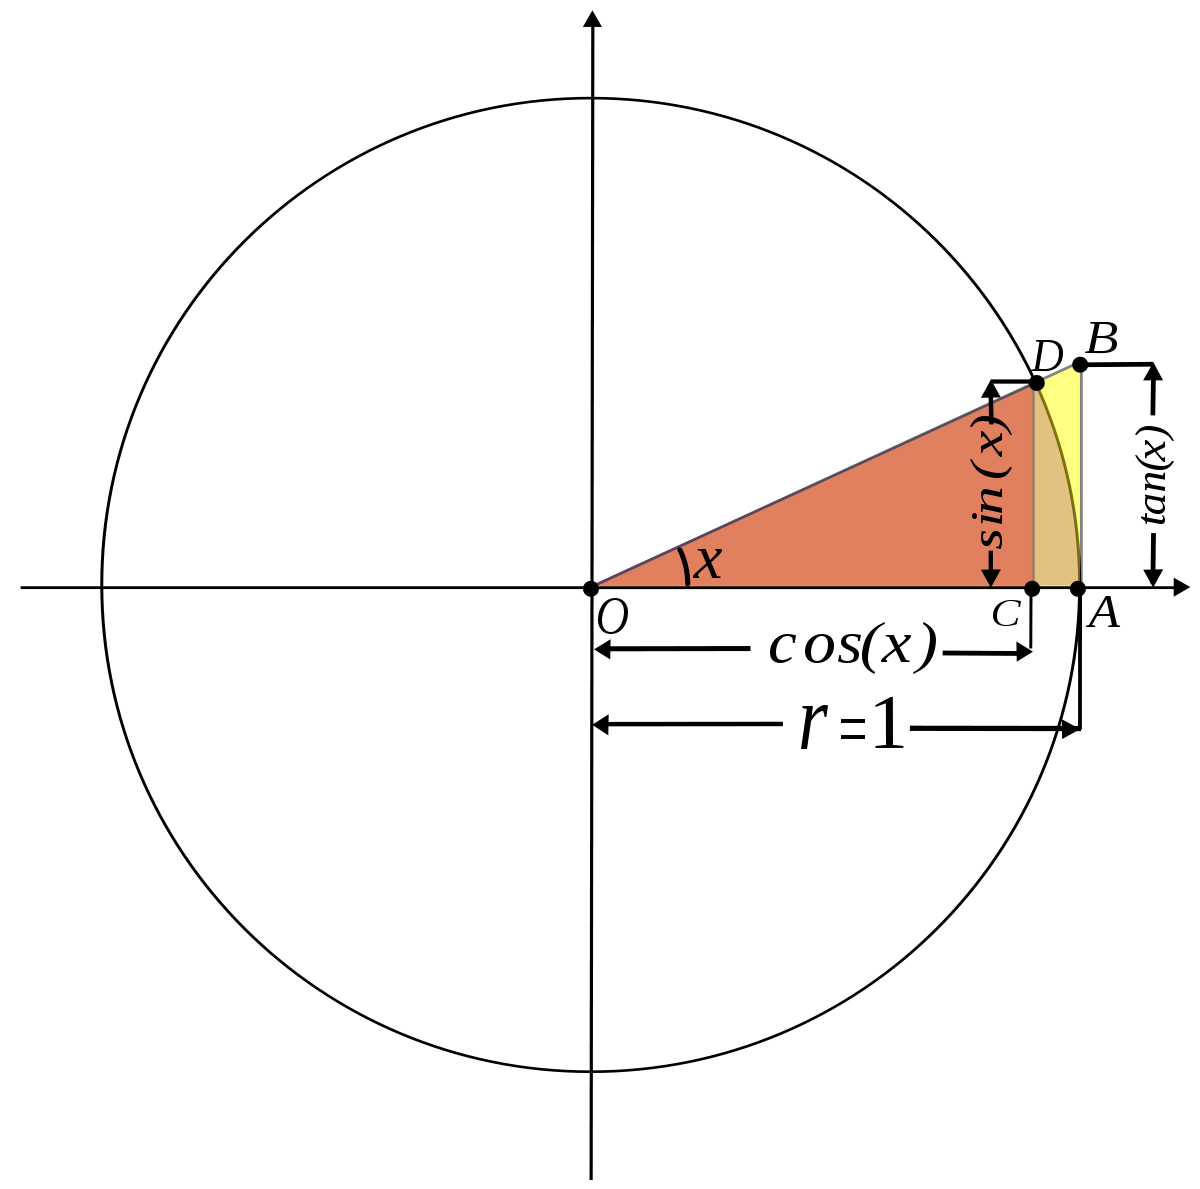
\includegraphics[width=0.35\textwidth]{circ_gon}
        \end{center}
        \[
            \cos:\mathbb{R} \rightarrow [-1,1]    
        \]
        \[
            \alpha \mapsto x_{p}    
        \]
        \[
            \sin:\mathbb{R} \rightarrow [-1,1]    
        \]
        \[
            \alpha \mapsto y_{p}    
        \]
        \subsubsection*{Proprietà}
            \begin{Large}
                \begin{itemize}
                    \item $\sin{(- \alpha)} = - \sin{\alpha}$
                    \item $\sin{(\pi - \alpha)} = \sin{\alpha}$
                    \item $\cos{(- \alpha)} = \cos{\alpha}$
                    \item $\cos{(\pi - \alpha)} = - \cos{\alpha}$
                    \item $|\sin{\alpha}| \leq 1, |\cos{\alpha}| \leq q$
                    \item $\cos$ è una funzione dispari, $\sin$ è una funzione pari
                    \item Dal teorema di pitagora: $\cos^{2}{\alpha} + \sin^{2}{alpha} = 1$
                \end{itemize}
            \end{Large}
        \subsubsection*{Formule}
            Siano $x_{1}, x_{2} \in \mathbb{R}\ \forall\ x_{1},x_{2} \in \mathbb{R}$
            \begin{Large}
                \begin{itemize}
                    \item $\cos{(x_{1} + x_{2})} = \cos{x_{1}} \cdot \cos{x_{2}} - \sin{x_{1} \cdot \sin{x_{2}}}$
                    \item $\sin{(x_{1} + x_{2})} = \sin{x_{1}} \cdot \cos{x_{2}} + \cos{x_{1} \cdot \sin{x_{2}}}$
                    \item $\cos{(2x)} = \cos^{2}{x} - \sin^{2}{x}$
                    \item $\sin{(2x)} = 2\sin{x}\cos{x}$
                    \item $|\cos{\frac{x}{2}}| = \sqrt{\frac{1 + \cos{x}}{2}}$
                    \item $|\sin{\frac{x}{2}}| = \sqrt{\frac{1 - \cos{x}}{2}}$
                \end{itemize}
            \end{Large}
    \subsubsection{Tangente}
        Sia $U$ una circonferenza goniometrica
        \begin{Large}
            \[
                \tan:\mathbb{R} \setminus \{\frac{\pi}{2} + k\pi, k \in \mathbb{Z}\} \rightarrow \mathbb{R}
            \]
            \[
                \alpha \mapsto y_{Q}    
            \]
        \end{Large}
        \begin{center}
            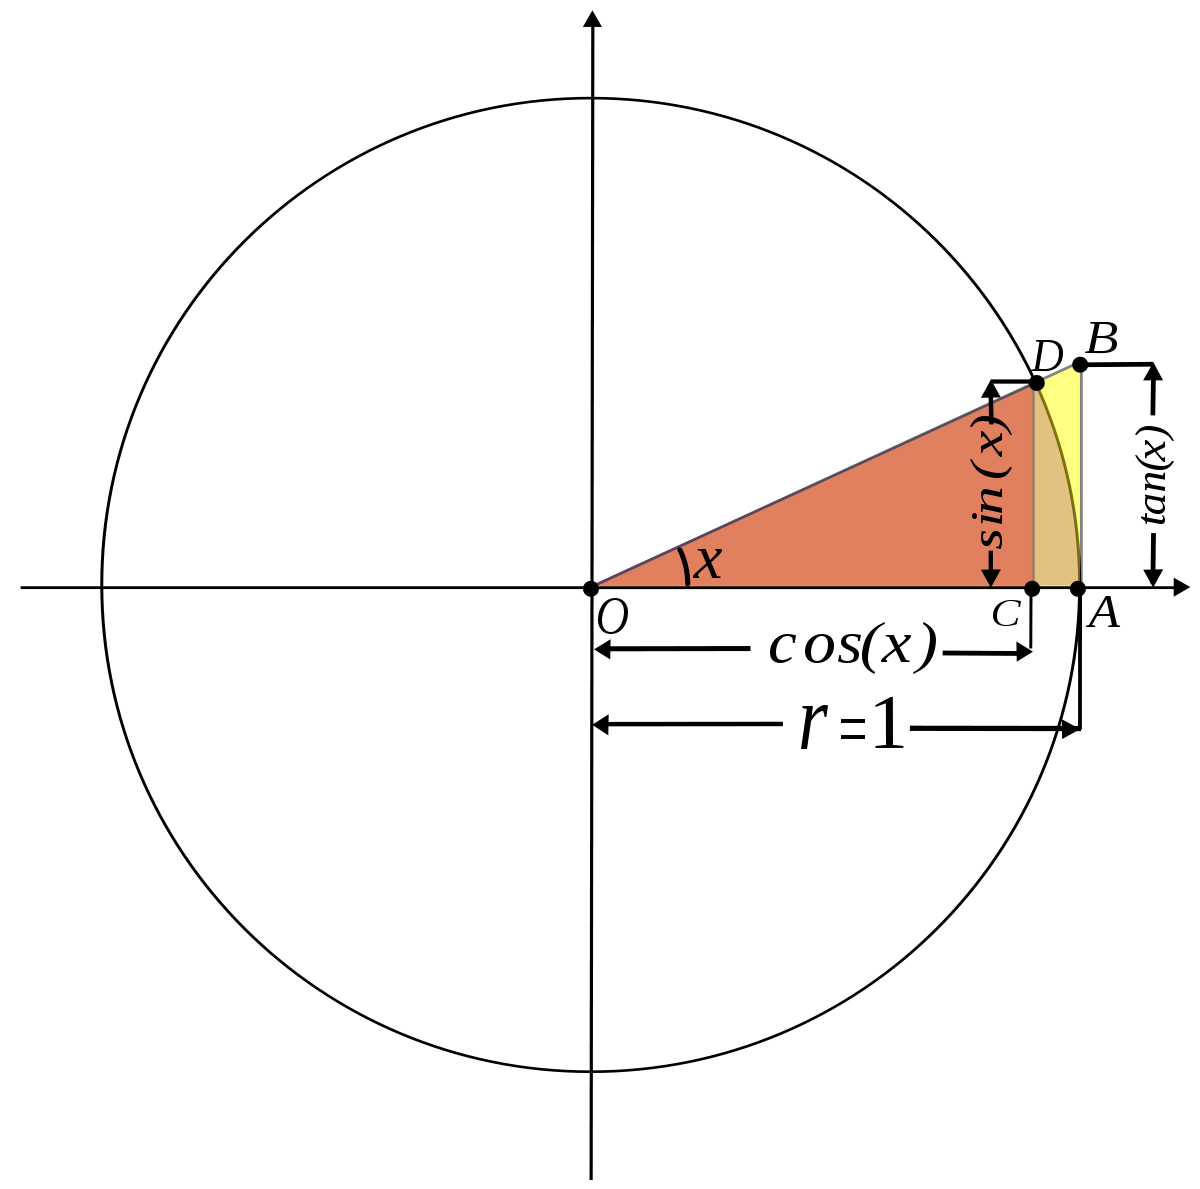
\includegraphics[width=0.35\textwidth]{circ_gon}
        \end{center}
        I triangoli $O\overset{\triangle}{P}H$ e $O\overset{\triangle}{Q}H$ sono simili, quindi:
        \[
            \frac{QK}{OK} = \frac{PH}{OH} \Rightarrow \frac{\tan{\alpha}}{1} = \frac{\sin{\alpha}}{\cos{\alpha}} \Rightarrow \tan{\alpha} = \frac{\sin{\alpha}}{\cos{\alpha}}    
        \]
        $\tan$ è periodica di periodo $\pi: \tan{(\alpha + \pi)} = \tan{\alpha}$. Dato che $\tan{\alpha}$ è una funzione dispari, e vista 
        la sua periodicità, è sufficiente studiarla solo nell'intervallo $[0, \frac{\pi}{2}[$.
        Analogamente, $cotan{\alpha} = \frac{\cos{\alpha}}{\sin{alpha}}$ (la retta è parallela all'asse $y$, passante per $(0,1)$ e si considera $x_{Q}$).
            

\end{document}